\documentclass[twocolumn,landscape,10pt]{article}
\usepackage[thinc]{esdiff} % for typesettign derivatives
\usepackage{amsthm} % provides an enhanced version of LaTex's \newtheorem command
\usepackage{mdframed} % framed environments that can split at page boundaries
\usepackage{enumitem} % bulletin points or other means of listing things
\usepackage{amssymb} % for AMS symbols
\usepackage{amsmath} % so as to use align
\usepackage{latexsym} % so as to use symbols like \leadsto
\usepackage{mathrsfs} % for using mathscr for char like operators
\usepackage{commath} % for using norm symbol
\usepackage{mathtools} % for using environments like dcases
\usepackage{authblk} % for writing affiliations
\usepackage{graphicx} % for importing images
\graphicspath{{./images/}} % for the path to images, also always put label behind captions
\usepackage{subfig}
\usepackage{textcomp} % for using degree symbol
\usepackage{hyperref} % for clickable link in the pdf & customizable reference text
\usepackage[all]{hypcap} % for clickable link to images instead of caption
\usepackage[margin=1.0in]{geometry} % default is 1.5in
% \usepackage[left=0.4in, right=0.4in, top=0.8in, bottom=0.8in]{geometry}
\usepackage[title]{appendix} % for attaching appendix
\allowdisplaybreaks % allow page breaking in display maths, like align
\usepackage{xcolor} % for setting color of a block of text, use \textcolor{<color>}{}
\usepackage[normalem]{ulem} % for strikethrough text, use \sout{}
% allow for more advanced table layout
\usepackage{booktabs}
\usepackage{multirow}
\usepackage{siunitx}
% for adjusting caption settings
\usepackage[justification=centering]{caption}
\captionsetup[table]{skip=10pt}

\theoremstyle{definition}
\mdfdefinestyle{defEnv}{%
  hidealllines=false,
  nobreak=true,
  innertopmargin=-1ex,
}

% The following is for writing block of code
\usepackage{listings}
\usepackage{color}

\definecolor{dkgreen}{rgb}{0,0.6,0}
\definecolor{gray}{rgb}{0.5,0.5,0.5}
\definecolor{mauve}{rgb}{0.58,0,0.82}

% setting of the thickness of the 4 lines of box
\setlength{\fboxrule}{2pt}

% Use the following to change code language and related settings
\lstset{frame=tb,
  language=Python,
  aboveskip=3mm,
  belowskip=3mm,
  showstringspaces=false,
  columns=flexible,
  basicstyle={\small\ttfamily},
  numbers=none,
  numberstyle=\tiny\color{gray},
  keywordstyle=\color{blue},
  commentstyle=\color{dkgreen},
  stringstyle=\color{mauve},
  breaklines=true,
  breakatwhitespace=true,
  tabsize=3,
  literate={~} {$\sim$}{1}
}

\pagestyle{headings}
\author{Lectured by Bernhard Kainz and Abhijeet Ghosh}
\title{Graphics}
\affil{Typed by Aris Zhu Yi Qing}
\begin{document}
\maketitle
\tableofcontents

\newpage
\section{Projections and Transformations}

\subsection{Parallel Projection}

\begin{itemize}
    \item For a vertex $\mathbf{V} = (V_x,V_y, V_z)^T$, the
        \underline{\textbf{projector}}
        (projection line) is defined by the parametric line equation
        \[
            \mathbf{P}=\mathbf{V}+\mu \mathbf{d}
        \]
    \item Assuming the projection plane is $z=0$, we can establish
        \[
            0 = P_z = V_z + \mu d_z
        \]
        to obtain $\mu$, thereby computing $P_x$ and $P_y$.
    \item \underline{\textbf{Orthographic projection}} is a special type of
        parallel projection:
        \begin{itemize}
            \item projection plane: $z=0$
            \item $\mathbf{d}=\begin{pmatrix}
                    0 & 0 & -1
                \end{pmatrix}^T$
            \item  $P_x=V_x$, $P_y=V_y$
        \end{itemize} 
\end{itemize} 

\subsection{Perspective Projections}

\begin{itemize}
    \item The \underline{\textbf{centre of projection}} is the viewpoint, which
        all the projectors pass through, assumed to be at the origin.
    \item For a vertex $\mathbf{V} = (V_x,V_y, V_z)^T$, the projector
        $\mathbf{P}$ has the equation
        \[
            \mathbf{P}=\mu\mathbf{V}
        \]
    \item Since the projection plane is at a constant $z$ value $f$, at the
        point of intersection we have
        \[
            f = P_z = \mu V_z
        \]
        to obtain $\mu$, thereby computing $P_x$ and $P_y$.
\end{itemize} 

\subsection{Space Transformations}

\subsubsection{Homogeneous Coordinates}

\begin{itemize}
    \item A \underline{\textbf{homogeneous coordinate}} is a three-dimensional
        coordinate with a fourth componenet called
        \underline{\textbf{ordinate}} which acts as a scale factor.
    \item Assuming a point $\mathbf{P}=(p_x,p_y,p_z)$ 
        in Cartesian coordinate, we introduce $s$ being the ordinate
        \[
            \mathbf{P}'=(p_x, p_y, p_z, s)
        \]
        to form a homogeneous coordinate.
    \item To convert $\mathbf{P}'$ back ot Cartesian, we will perform
        \underline{\textbf{perspective division}}
        \[
            \mathbf{P}''=\left(\frac{p_x}{s},\frac{p_y}{s},\frac{p_z}{s}\right),
        \]
        i.e.\ divide $x$, $y$ and $z$ values by the ordinate.
        Thus when $s=1$, $\mathbf{P}=\mathbf{P}''$.
    \item If $s\neq 0$, we have a \underline{\textbf{position vector}}.
        If $s=0$, we have a \underline{\textbf{direction vector}}.
\end{itemize} 

\subsubsection{Translation Matrix}

To apply a translation vector $\mathbf{t}=(t_x,t_y,t_z)$ to a point
$\mathbf{P}=(p_x,p_y,p_z)$, we do
\[
    \begin{pmatrix}
        1 & 0 & 0 & t_x \\
        0 & 1 & 0 & t_y \\
        0 & 0 & 1 & t_z \\
        0 & 0 & 0 & 1
    \end{pmatrix} 
    \begin{pmatrix}
        p_x \\
        p_y \\
        p_z \\
        1
    \end{pmatrix} 
    =
    \begin{pmatrix}
        p_x + t_x \\
        p_y + t_y \\
        p_z + t_z \\
        1
    \end{pmatrix} 
\]
with the inverse of the translation matrix as
\[
    \begin{pmatrix}
        1 & 0 & 0 & -t_x \\
        0 & 1 & 0 & -t_y \\
        0 & 0 & 1 & -t_z \\
        0 & 0 & 0 & 1
    \end{pmatrix}.
\]

\subsubsection{Scaling Matrix}

To scale a point from the origin, we can do
\[
    \begin{pmatrix}
        s_x & 0 & 0 & 0 \\
        0 & s_y & 0 & 0 \\
        0 & 0 & s_z & 0 \\
        0 & 0 & 0 & 1 \\
    \end{pmatrix} 
    \begin{pmatrix}
        p_x \\
        p_y \\
        p_z \\
        1
    \end{pmatrix} 
    =
    \begin{pmatrix}
        s_xp_x \\
        s_yp_y \\
        s_zp_z \\
        1
    \end{pmatrix} 
\]
with the inverse of the scaling matrix as
\[
    \begin{pmatrix}
        1/s_x & 0 & 0 & 0 \\
        0 & 1/s_y & 0 & 0 \\
        0 & 0 & 1/s_z & 0 \\
        0 & 0 & 0 & 1 \\
    \end{pmatrix} 
\]

\subsubsection{Rotation Matrix}

To rotate \underline{anti-clockwise} when looking \underline{along the direction} 
of the axis with a \underline{left-hand} axis system, we have
\[
    \mathcal{R}_x=
    \begin{pmatrix}
        1 & 0 & 0 & 0 \\
        0 & \cos{\theta} & -\sin{\theta} & 0 \\
        0 & \sin{\theta} & \cos{\theta} & 0 \\
        0 & 0 & 0 & 1
    \end{pmatrix}, \qquad
    \mathcal{R}_x^{-1}=
    \begin{pmatrix}
        1 & 0 & 0 & 0 \\
        0 & \cos{\theta} & \sin{\theta} & 0 \\
        0 & -\sin{\theta} & \cos{\theta} & 0 \\
        0 & 0 & 0 & 1
    \end{pmatrix},
\]
\[
    \mathcal{R}_y=
    \begin{pmatrix}
        \cos{\theta} & 0 & \sin{\theta} & 0 \\
        0 & 1 & 0 & 0 \\
        -\sin{\theta} & 0 & \cos{\theta} & 0 \\
        0 & 0 & 0 & 1
    \end{pmatrix}, \qquad
    \mathcal{R}_y^{-1}=
    \begin{pmatrix}
        \cos{\theta} & 0 & -\sin{\theta} & 0 \\
        0 & 1 & 0 & 0 \\
        \sin{\theta} & 0 & \cos{\theta} & 0 \\
        0 & 0 & 0 & 1
    \end{pmatrix}, 
\]
\[
    \mathcal{R}_z=
    \begin{pmatrix}
        \cos{\theta} & -\sin{\theta} & 0 & 0 \\
        \sin{\theta} & \cos{\theta} & 0 & 0 \\
        0 & 0 & 1 & 0 \\
        0 & 0 & 0 & 1
    \end{pmatrix} \qquad
    \mathcal{R}_z^{-1}=
    \begin{pmatrix}
        \cos{\theta} & \sin{\theta} & 0 & 0 \\
        -\sin{\theta} & \cos{\theta} & 0 & 0 \\
        0 & 0 & 1 & 0 \\
        0 & 0 & 0 & 1
    \end{pmatrix},
\]
to rotate along $x$, $y$ and $z$ axis respectively.
In other words, the right matrices are rotating clockwise.

\subsubsection{Projection Matrix}

For a perspective projection, placing the centre of projection at the origin and
using $z=f$ as before, we can use
\[
    \mathcal{M}_p=
    \begin{pmatrix}
        1 & 0 & 0 & 0 \\
        0 & 1 & 0 & 0 \\
        0 & 0 & 1 & 0 \\
        0 & 0 & 1/f & 0 \\
    \end{pmatrix} 
\]
For an orthographic projection, with the projection plane at $z=0$, we can use
\[
    \mathcal{M}_o=
    \begin{pmatrix}
        1 & 0 & 0 & 0 \\
        0 & 1 & 0 & 0 \\
        0 & 0 & 0 & 0 \\
        0 & 0 & 0 & 1 
    \end{pmatrix} 
\]

\section{Clipping}

\begin{itemize}
    \item \underline{\textbf{Clipping}} eliminates portions of objects outside
        the \underline{\textbf{viewing frustum}}, which is the boundaries of the
        image plane projected in 3D with a near and far clipping plane.
    \item \underline{Why} clipping?
        \begin{itemize}
            \item avoid degeneracy: e.g. don't draw objects behind the camera
            \item improve efficiency: e.g. do not process objects which are not visible.
        \end{itemize} 
    \item \underline{When} to clip?
        \begin{itemize}
            \item before perspective transform in 3D space:
                \begin{itemize}
                    \item 3D world space
                    \item use the equation of 6 planes
                    \item natural, not too degenerate
                \end{itemize} 
            \item in homogeneous coordinates after perspective transform 
                and \underline{before} perspective division:
                \begin{itemize}
                    \item clip space
                    \item canonical, independent of camera
                    \item simplest to implement, since clipping plane can align
                        with axis so that we can easily discard anything further
                        than the far plane or closer than the near plane
                \end{itemize} 
            \item in the transformed 3D screen space \underline{after} 
                perspective division:
                \begin{itemize}
                    \item Normalized Device Coordinates (NDC)
                    \item The regions extends from -1. to 1. in each axis.
                        Anything outside from the volume is discarded.
                    \item problem --- having negative orginates 
                \end{itemize} 
        \end{itemize} 
    \item \underline{\textbf{Halfspace}} We can define any plane as a test for a
        point $\mathbf{p}$:
        \[
            f(x,y,z)=\mathbf{H}\cdot \mathbf{p}=0
        \]
        where $\mathbf{H}=(H_x,H_y,H_z,H_s)$ and $\mathbf{p}=(x,y,z,1)$,
        such that 
        \[
            \begin{cases}
                \mathbf{H}\cdot \mathbf{p}>0  & \text{in one halfspace (pass-through)}\\
                \mathbf{H}\cdot \mathbf{p}<0 & \text{in the other halfspace (clip/cull/reject)}
            \end{cases} 
        \]
        \begin{itemize}
            \item \underline{\textbf{Segment Clipping}} Similarly we have
                \[
                    \begin{cases}
                        \mathbf{H}\cdot\mathbf{p}>0, \mathbf{H}\cdot\mathbf{q}<0
                        & \text{clip $\mathbf{q}$ to plane} \\
                        \mathbf{H}\cdot\mathbf{p}<0, \mathbf{H}\cdot\mathbf{q}>0
                        & \text{clip $\mathbf{p}$ to plane} \\
                        \mathbf{H}\cdot\mathbf{p}>0, \mathbf{H}\cdot\mathbf{q}>0
                        & \text{pass through} \\
                        \mathbf{H}\cdot\mathbf{p}<0, \mathbf{H}\cdot\mathbf{q}<0
                        & \text{clipped out}
                    \end{cases} 
                \]
            \item Test if an object is convex.
                \begin{enumerate}
                    \item For each face of the object, pick a random point.
                    \item For this point, compare with points from other faces,
                        check if
                        \[
                            \texttt{sign(f(xj,yj,zj)) != sign(f(xi,yi,zi))}
                        \]
                        then it is not convex.
                \end{enumerate} 
            \item Test if a point is contained in a concave object.
                \begin{itemize}
                    \item Cast a ray from the test point in any direction. If
                        the number of intersections with the object is odd, then
                        the test point is inside.
                \end{itemize} 
        \end{itemize} 
\end{itemize} 

\section{Graphics Pipeline}

\subsection{Application}

\begin{itemize}
    \item executed by the software on the main processor (CPU)
    \item typical tasks performed: collision detection, animation, morphing,
        perform spatial subdivision scheme (quadtree, octree).
    \item to reduce the amount of main memory required at a given time
\end{itemize} 

\subsection{Geometry}

\begin{enumerate}
    \item Modelling Transformations
    \item Illumination (Shading)
    \item Viewing Transformations (Perspective/Orthographic)
    \item Clipping
    \item Projection (to screen space --- window-viewport transformation)
\end{enumerate} 

\subsection{Rasterization}

\begin{itemize}
    \item \underline{\textbf{Rasterization}} is the task of taking an image 
        described in a vector graphics format (shapes) and 
        converting it into a raster image (a series of pixels).
    \item During this process, fragments/raster points are created from 
        continuous primitives.  A \underline{\textbf{fragment}} 
        can be thought of as the data needed to shade the pixel 
        (e.g. color, illumination, texture) 
        and to test whether the fragment survives to become a pixel 
        (depth, alpha, etc.)
    \item Eventually, one or more fragments are merged to become a
        \underline{\textbf{pixel}}, which is the smallest addressable element
        in a raster image.
    \item To prevent from exposing the process of gradual screening of the
        primitives, double buffering is used so that 
        the rasterization takes place in a special memory,
        and as soon as the image is completely rastered, 
        it is copied into the visible area of the image memory (frame buffer).
\end{itemize} 

\subsection{Shading}
\underline{\textbf{Shading}} refers to the modification of individual 
vertices or fragments within the graphics pipeline.
This is the \emph{programmable} part of the graphics pipeline.

\subsubsection{Vertex Shader}
\begin{itemize}
    \item executed once for each vertex
    \item only has access to the vertex and no neighbouring vertices,
        the topology, or similar
\end{itemize} 

\subsubsection{Tessellation Shader}
\begin{itemize}
    \item divides an area (triangle or square) into smaller areas
    \item advantage: allow detail to be dynamically added and subtracted
        from a 3D polygon mesh and its silhouette edges based on control
        parameters (e.g. camera distance)
    \item The \underline{\emph{Tessellation Control Shader}} (TCS) determines
        how much tessellation to do. It is optional; default
        tessellation values can be used.
    \item The \underline{\emph{tessellation primitive generator}} 
        (not programmable) takes the input patch 
        and subdivides it based on values computed by the TCS.
    \item The \underline{\emph{Tessellation Evaluation Shader}} (TES) takes the
        tessellated patch and computes the vertex values for each
        generated vertex.
\end{itemize} 

\subsubsection{Geometry Shader}
\begin{itemize}
    \item takes a single primitive as input and may output zero or more
        primitives of the same type
    \item has access to multiple vertices, if the primitive consists of multiple
        vertices
    \item A \underline{\textbf{primitive}} can mean
        \begin{enumerate}[label = (\alph*)]
            \item the interpretation scheme to determine what a stream
                of vertices represents when being rendered,
                which can be arbitrarily long
            \item the \emph{result} of the interpretation of a vertex
                stream (also called the \underline{\emph{base primitive}})
        \end{enumerate} 
    \item Use case: in a particle system, the inputs are processed
        points, and geometry shader generates polygons/cubes/etc. to
        save computation in the previous pipelines.
\end{itemize} 

\subsubsection{Fragment Shader}

\begin{itemize}
    \item executed once for every fragment generated by the rasterization
    \item it takes in interpolated vertex attributes
    \item it calculates the color of the corresponding fragment
\end{itemize} 

\section{OpenGL}

\begin{itemize}
    \item The interface is platform independent, but the implementation is
        platform dependent.
    \item It defines an abstract rendering device and a set of functions to
        operate the device.
    \item It is a low-level ``immediate mode'' graphics API with drawing
        commands and no concept of permanent objects, operating as a state
        machine.
    \item To write an OpenGL programme, we need to
        \begin{enumerate}
            \item create a render window via library such as glut, Qt, etc.
            \item setup viewport, model transformation and file I/O (shader,
                textures, etc.)
            \item implement frame-generataion (update/rendering) functions 
                to define what happens in every frame
        \end{enumerate} 
    \item Basic concepts:
        \begin{itemize}
            \item \underline{\textbf{Context}}
                \begin{itemize}
                    \item represents an instance of OpenGL
                    \item a process can have multiple contexts to share
                        resources
                    \item one-to-one mapping between a context and a thread
                \end{itemize} 
            \item \underline{\textbf{Resources}}
                \begin{itemize}
                    \item act as sources of input and sinks for output
                    \item e.g. texture images(input), buffers(output)
                \end{itemize} 
            \item \underline{\textbf{Object Model}}
                \begin{itemize}
                    \item Object instances are identified by unique names
                        (unsigned integer handle).
                    \item Commands work on targets, where each target is bounded
                        by an object.
                \end{itemize} 
        \end{itemize} 
    \item \underline{\textbf{Buffer objects}} are regular OpenGL objects that
        store an array of unformatted memory allocated by the OpenGL context
        (i.e.\ GPU).
    \item has primitive types such as \texttt{GL\_POINTS}, \texttt{GL\_LINES},
        \texttt{GL\_POLYGONS}, \texttt{GL\_TRIANGLES}, etc.
\end{itemize} 

\section{Illumination and Shading}

\subsection{Physics of Shading}

\begin{itemize}
    \item object properties
        \begin{itemize}
            \item the position of the object relative to the light sources
            \item the surface normal vector
            \item the albedo of the surface (ability to absorb light energy) and
                the reflectivity of the surface
        \end{itemize} 
    \item light source properties
        \begin{itemize}
            \item intensity of the emitted light
            \item distance to the point on the surface
        \end{itemize} 
    \item energy (Joule) of a photon is
        \[
            e(\lambda) = \frac{hc}{\lambda}
        \]
        where $h\approx 6.63\times 10^{-34}J\cdot s$ and $c\approx 3\times
        10^{8}m/s$.
    \item radiant energy (Joule) of $n$ photons is
        \[
            Q = \sum_{i=1}^{n} e(\lambda_i)
        \]
    \item Radiation/radiant/electromagnetic flux (Watts) is
        \[
            \Phi=\frac{\mathrm{d} Q}{\mathrm{d}t}
        \]
    \item \underline{\textbf{Radiance}} (Watt/($\text{meter}^{2}\,\cdot$ steradian)) 
        is density of a incident flux falling onto a surface 
        \underline{in a particular direction}
        \[
            L(\omega)=\frac{\mathrm{d}^2\Phi}{\cos{\theta}\;\mathrm{d}A\mathrm{d}\omega}
        \]
    \item \underline{\textbf{Irradiance}} (Watt/$\text{meter}^{2}$) 
        is density of the incident flux falling onto a surface
        \[
            E=\frac{\mathrm{d}\Phi}{\mathrm{d}A}
        \]
    \item  We define the
        \underline{\textbf{Bidirectional Reflectance Distribution Function}}
        (BRDF) (1/steradian)
        \[
            f_r(\theta_i,\phi_i,\theta_r,\phi_r)=
            f_r(\omega_i,\omega_r)=\frac{\mathrm{d}L_r(\omega_r)}{\mathrm{d}E_i(\omega_i)}
        \]
        by ignoring other physical phenomenon such as absorption,
        transmission, fluorescence, diffraction, etc.
        \begin{itemize}
            \item \underline{\emph{Isotropic BRDF}} is such that rotation along
                surface normal does not change reflectance.
            \item \underline{\emph{Anisotropic BRDF}} changes reflectance when
                rotating along surface normal, which happens on surfaces with
                strongly oriented microgeometry elements such as brushed metals,
                hair, cloth, etc.
            \item non-negativity: $f_r(\omega_i,\omega_r)\ge 0$
            \item energy conservation: $\forall\omega_i, \int_\Omega
                f_r(\omega_i,\omega_r)\cos{\theta_r}\mathrm{d}\omega_r\le 1$
            \item reciprocity: $f_r(\omega_i,\omega_r)=f_r(\omega_r,\omega_i)$
        \end{itemize} 
    \item To compute the reflected radiance discretely, with $n$ points light
        sources, we have
        \[
            L_r(\omega_r)=\sum_{i=1}^{n} f_r(\omega_i,\omega_r)E_i
            =\sum_{i=1}^{n}
            f_r(\omega_i,\omega_r)\cos{\theta_i}\frac{\Phi_i}{4\pi d_i^2}
        \]
    \item Ideally, BRDF is constant, so with a single point light source
        \[
            L(\omega_r)=k_d(n\cdot l) \frac{\Phi_s}{4\pi d^2}
        \]
        where $k_d$ is the diffuse reflection coefficient,
        $n$ is the (normalized) surface normal,
        and $l$ is the (normalized) light direction from surface.
\end{itemize} 

\subsection{The Phong Model}

\begin{itemize}
    \item light sources are assumed to be point-shaped, i.e.\ no spatial extent
    \item Reflected radiance calculation is
        \[
            L(\omega_r) = k_s{(v\cdot r)}^{q}\frac{\Phi_s}{4\pi d^2}
            = k_s{(v\cdot (2(n\cdot l)n - l))}^{q}\frac{\Phi_s}{4\pi d^2}
        \]
        where $k_s$ is the specular reflection coefficient, $q$ is the specular
        reflection exponent, $v$ is the direction vector from surface to camera,
        and $r$ is the reflected ray.
    \item Blinn-Phong variation is that
        \[
            L(\omega_r) = k_s{(n\cdot h)}^{q}\frac{\Phi_s}{4\pi d^2}
            \qquad\text{with}\qquad
            h=\frac{l+v}{\norm{l+v}}
        \]
    \item The Phong model is the sum of three components: diffuse, specular and
        ambient, i.e.\
        \[
            L(\omega_r)=k_a + \left(k_d(n\cdot l)+k_s{(v\cdot r)}^{q}\right)
            \frac{\Phi_s}{4\pi d^2}
        \]
    \item Sometimes using $(d+s)$ instead of $d^2$ produces better result, where
        $s$ is a heuristic constant.
\end{itemize} 

\subsection{Shading}

\subsubsection{Flat Shading}

\begin{itemize}
    \item each polygon is shaded uniformly over its surface
    \item computed by taking a point in the center and at the surface normal
    \item normally only the diffuse and ambient components are used
\end{itemize} 

\subsubsection{Gouraud Shading}

\begin{itemize}
    \item interpolate color using shade value at each vertex
    \item can interpolate intensity at each vertex from all the polygons that
        meet at that vertex to create the impression of a smooth surface
    \item cannot accurately model specular components,
        since we don't have normal vector at each point on a polygon
\end{itemize} 

\subsubsection{Phong Shading}

\begin{itemize}
    \item interpolate normals across triangles at fragment stage
    \item more accurate modelling of specular components, but slower
\end{itemize} 


\section{Color}

\subsection{RGB CIE Color Space}

\begin{itemize}
    \item a standard normalized representation of colors
        ranging from 0 to 1, with
        \[
            x=\frac{r}{r+g+b},y=\frac{g}{r+g+b},z=\frac{b}{r+g+b}=1-x-y
        \]
    \item the actual visible colors are a subset of this as shown in Figure
        \ref{fig:cie},
        done through manual testing
        \begin{figure}
          	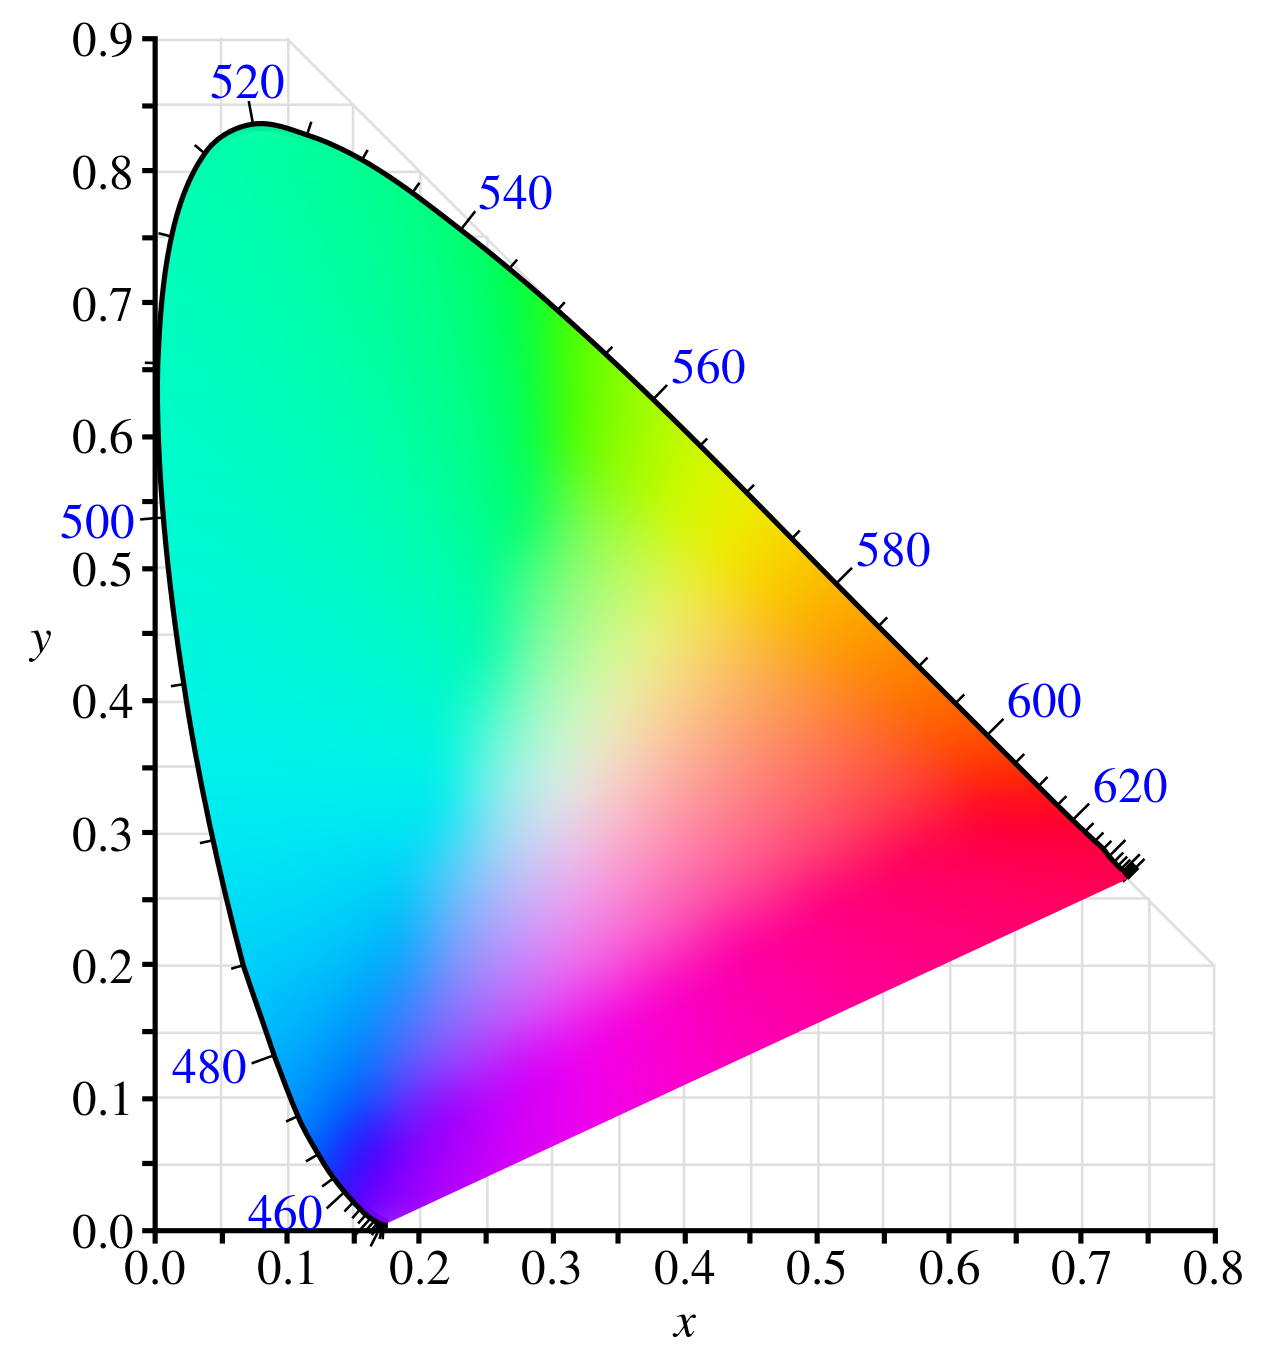
\includegraphics[scale=0.20]{cie.png}
          	\centering
          	\caption{The CIE 1931 color space. Red is at $(0.628,0.346,0.026)$,
            Green is at $(0.268, 0.588,0.144)$, Blue is at $(0.150,0.07,0.780)$}\label{fig:cie}
        \end{figure}
        
    \item the shape must be convex, since any blend (interpolation) of pure
        colors should create a color in the visible region.
    \item the \underline{\textbf{pure colors}} are around the edge of the
        diagram, also called \underline{\textbf{fully saturated}}
    \item the line joining purple and red has no pure equivalent; the colours
        can only be created by blending
    \item \underline{\textbf{Saturation}} of an arbitrary point is the ratio of
        its distance to the white point over the distance of the white point to
        the edge.
    \item white point: when $x=y=z=0.\dot{3}$
    \item The \underline{\textbf{complement color}} of a color is the point
        diametrically opposite through the white point. Computationally, if the
        color has value $(r,g,b)$, its complement color is
        $(255-r,255-g,255-b)$.
    \item The \underline{\textbf{additive primaries}} are RGB (Red, Green, Blue)
        and the \underline{\textbf{subtractive primaries}} are CMY (Cyan,
        Magenta, Yellow).
        Red is the complement color of Cyan, and similarly for Green and Blue,
        as shown in Figure \ref{fig:primaries}.
        \begin{figure}
          	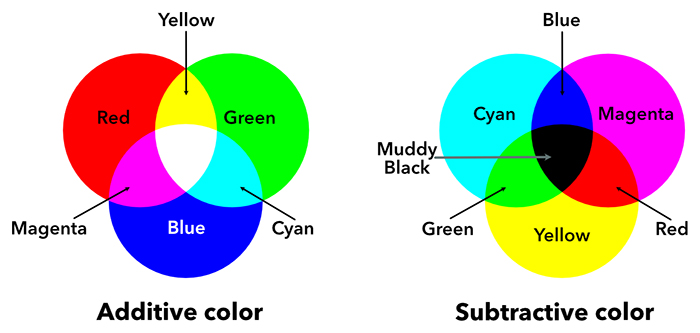
\includegraphics[scale=0.55]{primaries.png}
          	\centering
          	\caption{additive and subtractive primaries}\label{fig:primaries}
        \end{figure}
    \item RGB can be converted to CIE by
        \[
            \begin{pmatrix}
                x \\
                y \\
                z
            \end{pmatrix} 
            =
            \begin{pmatrix}
                0.628 & 0.268 & 0.15 \\
                0.346 & 0.588 & 0.07 \\
                0.026 & 0.144 & 0.78
            \end{pmatrix} 
            \begin{pmatrix}
                r \\
                g \\
                b
            \end{pmatrix} 
        \]
\end{itemize} 

\subsection{HSV Color Representation}

\begin{itemize}
    \item \underline{\textbf{Hue}} corresponds notionally to pure color
    \item \underline{\textbf{Saturation}} is the proportion of pure color
    \item \underline{\textbf{Value}} is the brightness/intensity
    \item We can visualize the perceptual color space in HSV as in Figure
        \ref{fig:hsv}.
        \begin{figure}
            \centering
            \subfloat[][The conical representation of the HSV model]{ 
                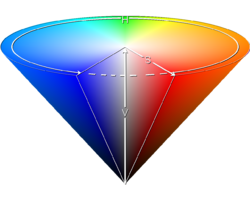
\includegraphics[scale=0.55]{hsv1.png}
            }
            \subfloat[][The HSV color wheel]{ 
                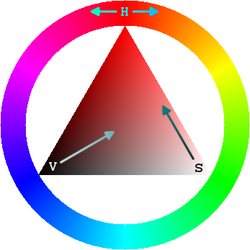
\includegraphics[scale=0.55]{hsv2.png}
            }
          	\caption{HSV model}\label{fig:hsv}
        \end{figure}
    \item Conversion between RGB and HSV can be done as
        \begin{align*}
            V & = \text{max}(r, g, b) \\
            S & = \frac{\text{max}(r,g,b)-\text{min}(r,g,b)}{\text{max}(r,g,b)}\\
            H & = 
            \begin{cases}
                \text{undefined} & r=g=b \\
                120\cdot \dfrac{g-b}{(r-b)+(g-b)} & (r>b)\wedge(g>b) \\[8px]
                120 + 120\cdot \dfrac{b-r}{(g-r)+(b-r)} & (g>r)\wedge(b>r) \\[8px]
                240 + 120\cdot \dfrac{r-g}{(r-g)+(b-g)} & (r>g)\wedge(b>g)
            \end{cases} 
        \end{align*} 
\end{itemize} 

\subsection{Transparancy}

We can model transparency with an $\alpha$ channel, with
\begin{itemize}
    \item transparent: $\alpha=0$
    \item semi-transparent: $0<\alpha<1$
    \item opaque: $\alpha=1$
\end{itemize} 
Suppose that we put $A$ over $B$ over background $G$,
\begin{itemize}
    \item How much of $B$ is blocked by $A$? $\alpha_A$
    \item How much of $B$ shows through $A$? $(1-\alpha_A)$
    \item How much of $G$ shows through both $A$ and $B$? $(1-\alpha_A)(1-\alpha_B)$
    \item How much does $G$ contribute to the overall color?
        $(1-\alpha_A)(1-\alpha_B)\alpha_G$
\end{itemize} 


\section{Texture}

\subsection{Definition}

\begin{itemize}
    \item \underline{\textbf{Texture (map)}} is an image applied (mapped)
        to the surface of a shape or polygon.
    \item A texture can be 1D, 2D, or 3D, but 2D is the most common for visible
        surfaces.
    \item \underline{\textbf{Raster images}} are 2D rectangular matrices or grid
        of square pixels, often used as textures.
    \item \underline{\textbf{Procedural texture}} is a texture created using a
        mathematical description rather than directly stored data 
        (e.g. raster image). Mathematically, it is a function $f$ defiend as
        \[
            f:\mathbf{p}\mapsto\text{color},
        \]
        where $\mathbf{p}$ is a coordinate.
        \begin{itemize}
            \item[+] Very small memory footprint before the texture map is
                generated. The ultimate way in image compression.
            \item[+] No texture memory is really needed since generated ``on the
                fly'' in a fragment shader, resulting in the exactly right level
                of detail for each pixel on the screen.
            \item[-] Hard to get a formula to get the exact/natural look.
            \item[-] On-the-fly generation can take a lot of shader
                program instructions, almost always slower than just
                loading/looking up one.
        \end{itemize} 
\end{itemize} 

\subsection{Photo Textures Mapping}

\subsubsection{Mechanism}

\begin{itemize}
    \item Define a 2D coordinate system on an image mapped onto a 3D object.
    \item For each fragment on an object's surface, work out what coordinate 
        needs to be sampled in the image's 2D space to get the right color.
    \item Conventionally, texture coordinates are denoted with $(s,t)$ 
        (\emph{texture space}). Canonically it goes from (0,0) to (0,1).
        The object surface is denoted with $(u,v)$ (\emph{object space}) 
        and the pixel on the screen is denoted with $(x,y)$ (\emph{screen space}).
        We need to define
        \[
            \text{\underline{\textbf{Parameterization}}}:(s,t)\mapsto(u,v)
        \]
        which is the process of finding parametric equations of textures and
        objects so that texture can be mapped onto object surface, and
        \[
            \text{\underline{\textbf{Rendering}}}:(u,v)\mapsto(x,y)
        \]
        which is the process of generating an image from a model.
\end{itemize} 

\subsubsection{Parameterization}

\begin{itemize}
    \item \underline{Planar mapping}: ignore one of the coordinates
    \item \underline{Cylindrical/Spherical mapping}: compare to
        cylindrical/spherical coordinate systems
    \item \underline{Box mapping}: 6 planar mapping
    \item \underline{\textbf{Unwrapping}}: the process of creating manual
        mapping
\end{itemize} 

\subsubsection{Texture Addressing (Mode)}

What happens outside $[0,1]$?
Following the order in Figure \ref{fig:texture_addressing},
\begin{itemize}
    \item \underline{static color}: we use a static color
        (red in this case)
    \item \underline{clamped}: we use the last color in the range
    \item \underline{repeated}: wrap back to the first coordinate, repeating the
        texture
    \item \underline{mirrored}: similar to repeated, but go backwards insteads
        after ending the texture
\end{itemize} 

\begin{figure}
  	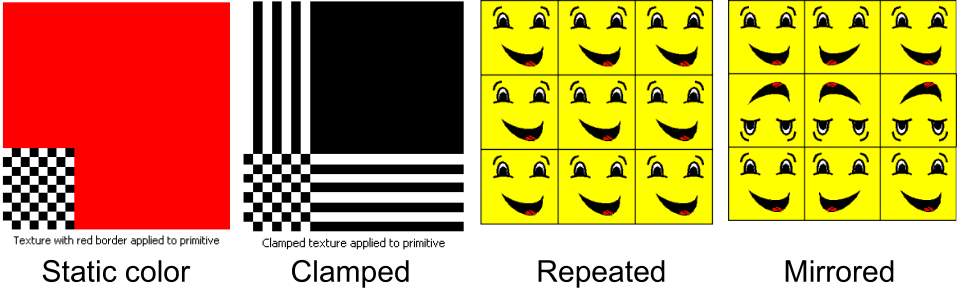
\includegraphics[scale=0.30]{texture_addressing.png}
  	\centering
  	\caption{Different texture addressing}\label{fig:texture_addressing}
\end{figure}


\subsection{Perspective Correct Interpolation}

\begin{itemize}
    \item cannot simply perform linear interpolation as in Gouraud shading on
        texture coordinates
    \item The problem:
        \begin{itemize}
            \item perspective projection \underline{\textbf{does not preserve}}
                linear combinations of points
            \item e.g. equal distances in 3D do not
                map to equal distances in screen space, as shown in figure
                \ref{fig:inter_err}.
        \end{itemize} 
        \begin{figure}
          	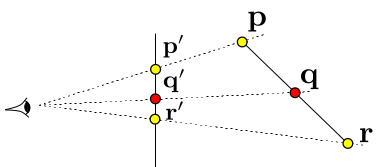
\includegraphics[scale=0.55]{interpolation_error.png}
          	\centering
          	\caption{perspective interpolation error}\label{fig:inter_err}
        \end{figure}
    \item The solution: 
        \begin{itemize}
            \item Assume image plane is at $z=f=1$.
            \item Let $t$ controls linear blend of texture coordinates of
                $\mathbf{p}$ and $\mathbf{r}$ and let 
                \[
                    t_p=0,\; t_r=1.
                \]
            \item  Let $\text{lerp}(x,y)$
                be the linear interpolation function, and as such
                \[
                    t_q=t_{q'}z_q=
                    \frac{\text{lerp}(t_{p'},t_{r'})}{\frac{1}{z_q}}=
                    \frac{\text{lerp}(\frac{t_p}{z_p},\frac{t_r}{z_r})}{\text{lerp}(\frac{1}{z_p},\frac{1}{z_r})}
                \]
        \end{itemize} 
    \item The algorithm: given texture parameter $t$ at vertices,
        \begin{enumerate}
            \item compute $\frac{1}{z}$ for each vertex
            \item linearly interpolate $\frac{1}{z}$ across the triangle
            \item linearly interpolate $\frac{t}{z}$ across the triangle
            \item perform perspective division via dividing $\frac{t}{z}$ by
                $\frac{1}{z}$ to obtain $t$
        \end{enumerate} 
\end{itemize} 

\subsection{Texture Mapping and Illumination}

\begin{itemize}
    \item For texture-mapped object, changing the lighting will not show the
        unevenness of the object's surface.
    \item \underline{\textbf{Bump mapping}}: textures to alter the surface
        normal of an object. Shading on the object is changed, but its
        silhouette is not.
    \item \underline{\textbf{Displacement mapping}}: textures to change the
        shading of both the object and its silhouette. It actually moves the
        surface point --- geometry is displaced before determining visibility.
    \item \underline{\textbf{Environment mapping}}: we can simulate reflections
        by using the direction of the reflected ray to index a spherical texture
        map at ``infinity''.
\end{itemize} 

\section{Rasterization, Visibility, and Anti-aliasing}

\subsection{Background}

\begin{itemize}
    \item \underline{\textbf{Rasterization}} determines which pixels are drawn
        into the framebuffer.
    \item Pixels have unique framebuffer location, but multiple fragments can be
        at the same address.
    \item \underline{\textbf{Alias effects}}: an unreal visual artefacts 
        caused by undersampling e.g. straight lines look jagged.
\end{itemize} 

\subsection{Barycentric Coordinates}

\begin{itemize}
    \item let vertices of a triangle be $\mathbf{a}$, $\mathbf{b}$, and $\mathbf{c}$,
        then any point $\mathbf{p}$ can be specified in the plane as
        \begin{align*}
            \mathbf{p}
            &=\mathbf{a}+\beta(\mathbf{b}-\mathbf{a})+\gamma(\mathbf{c}-\mathbf{a})
            =(1-\beta-\gamma)\mathbf{a}+\beta \mathbf{b}+\gamma \mathbf{c} \\
            &=\alpha \mathbf{a}+\beta \mathbf{b}+\gamma \mathbf{c},
        \end{align*} 
        and $(\alpha,\beta,\gamma)$ is called (absolute) barycentric coordinates.
    \item If $\mathbf{p}$ is inside the triangle
        $(\mathbf{a},\mathbf{b},\mathbf{c})$, we have $0<\alpha,\beta,\gamma<1$;
        if $\mathbf{p}$ is on an edge, one coefficient is 0;
        if $\mathbf{p}$ is on a vertex, one coefficient is 1.
    \item Since implicit equation in 2D is defined as
        \[
            f(x,y)=Ax+By+c=0
        \]
        and an implicit line through $(x_a,y_a)$ and $(x_b,y_b)$ is
        \[
            f_{ab}(x,y)=(y_a-y_b)x+(x_b-x_a)y+x_ay_b-x_by_a=0,
        \]
        note that a barycentric coordinate such as $\beta$ is a
        \underline{\textbf{signed distance}} from a line 
        (in this case, the line through $\mathbf{a}$ and $\mathbf{c}$),
        and we can use implicit line equations to evaluate the signed distance,
        we have
        \[
            \frac{f_{ac}(x_b,y_b)}{f_{ac}(x,y)}=\frac{1}{\beta}
            \Longrightarrow
            \beta=\frac{f_{ac}(x,y)}{f_{ac}(x_b,y_b)}
        \]
        and we can obtain similar results for $\alpha$ and $\gamma$, thereby
        computing the barycentric coordinates with the given cartesian coordinates.
    \item In general, the barycentric coordinates for $\mathbf{p}$ are the
        solution of the linear system
        \[
            \begin{pmatrix}
                x_a & x_b & x_c \\
                y_a & y_b & y_c \\
                1 & 1 & 1
            \end{pmatrix} 
            \begin{pmatrix}
                \alpha \\
                \beta \\
                \gamma
            \end{pmatrix} 
            =
            \begin{pmatrix}
                x \\
                y \\
                1
            \end{pmatrix} 
        \]
    \item Let $a,b,c$ be the side lengths of the triangle,
        from barycentric to trilinear coordinates:
        \[
            (\alpha,\beta,\gamma)\mapsto(\frac{\alpha}{a},\frac{\beta}{b},\frac{\gamma}{c}),
        \]
        from trilinear to barycentric coordinates:
        \[
            (t_1,t_2,t_3)\mapsto(t_1a,t_2b,t_3c)
        \]
    \item \underline{\textbf{Triangle Rasterization}}:
        we can check if ($0<\alpha,\beta,\gamma<1$) to determine if
        a fragment of a triangle should be generated.
\end{itemize} 

\subsection{Visibility}

\begin{itemize}
    \item \underline{\textbf{Painter's algorithm}}: sort the triangles using the
        $z$ values in camera space and draw them from back to front.
        \begin{itemize}
            \item[-] not efficient due to costly sorting
            \item[-] suffer from correctness issues such as intersections,
                cycles, etc.
        \end{itemize} 
    \item \underline{\textbf{depth buffer (z-buffer)}}: perform hidden surface
        removal per-fragment by saving the $z$ value for each fragment and keep
        only the fragment with the smallest $z$ value at each pixel. Use
        \underline{\emph{z-buffer (2D buffer)}} of the same size as image to
        save $z$ values.
        \begin{itemize}
            \item[+] facilitates hardware implementation
            \item[+] handles intersections and cycles
            \item[+] draw opaque polygons in any order
        \end{itemize} 
\end{itemize} 

\subsection{Anti-aliasing}

\begin{itemize}
    \item apply a degree of blurring to the boundary such that the
        aliasing effect is reduced.
    \item \underline{\textbf{Supersampling}}
        \begin{enumerate}
            \item Compute the picture at a high resolution to that of the
                display area.
            \item Supersamples are averaged to find the pixel value.
            \item This blurs the boundaries and leaves the coherent areas of
                color unchanged.
        \end{enumerate} 
    \item \underline{\textbf{Convolution filtering}}: use a filter that takes a
        (weighted) average over a small region around the pixel to blur the
        image, such as
        \[
            \frac{1}{36}
            \begin{pmatrix}
                1 & 4 & 1 \\
                4 & 16 & 4 \\
                1 & 4 & 1
            \end{pmatrix} 
        \]
        \begin{itemize}
            \item[+] very fast, can be done in hardware
            \item[+] generally applicable
            \item[-] degrade the image while enhancing its visual appearance
        \end{itemize} 
\end{itemize} 


\section{Ray Tracing}

\subsection{Introduction}

\begin{itemize}
    \item \underline{\textbf{Direct illumination}}: a surface point receives
        light directly from all light sources in the scene.
    \item \underline{\textbf{Global illumination}}: a surface point receives
        light after the light rays interact with other objects in the scene. 
        \begin{itemize}
            \item points may be in shadow
            \item rays may refract through transparent material
            \item computed by reflection and transmission rays
        \end{itemize} 
    \item Ray tracing pros and cons
        \begin{itemize}
            \item[+] Easy to implement
            \item[+] extends well to global illumination, such as shadows,
                reflections/refractions, etc.
            \item[-] speed --- seconds/frame, instead of frames/second
        \end{itemize} 
\end{itemize} 

\subsection{Basic Ray Tracing Algorithm}

\begin{enumerate}
    \item cast one ray per pixel
    \item\label{rt-step-2} compute nearest intersection with an object in the scene
    \item check if the ray from the intersection point to the light source is
        occluded
        \begin{itemize}
            \item if occlusion happens, stop tracing
            \item if no occlusion, compute color at the intersection point,
                update ray to be the next ray to be traced, and go back to step \ref{rt-step-2}.
        \end{itemize} 
\end{enumerate} 

\subsection{Mathematical Computations}

\subsubsection{Reflected Ray}

Givne that $\mathbf{v}$ is the primary ray, $\mathbf{n}$ is the unit surface
normal, we can compute the reflected ray $\mathbf{v}'$ as
\[
    \mathbf{v}'=\mathbf{v}-(2\mathbf{v}\cdot\mathbf{n})\mathbf{n}.
\]

\subsubsection{Color computation}

We can compute color/shadow as
\[
    L = k_a+s\left[k_d(\mathbf{n}\times \mathbf{l})
    +k_s{(\mathbf{v}\times \mathbf{r})}^{q}\right]I_s
    +k_\text{reflected}L_\text{reflected}+k_\text{refracted}L_\text{refracted}
\]
where
\[
    s =
    \begin{cases}
        0 & \text{if light source is obscured} \\
        1 & \text{if light souce is not obscured}.
    \end{cases} 
\]
We can use multiple shadow rays to sample an area light source, allowing us to
create \emph{soft shadows}.

\subsubsection{Refraction}

\begin{itemize}
    \item The angle of the refracted ray can be determined by the Snell's law
        \[
            \eta_1\sin{\phi_1}=\eta_2\sin{\phi_2}
        \]
        where
        \begin{itemize}
            \item $\eta_1$ is the refractive index for medium 1
            \item $\eta_2$ is the refractive index for medium 2
            \item $\phi_1$ is the angle between the incident ray and the surface normal
            \item $\phi_2$ is the angle between the refracted ray and the surface normal
        \end{itemize} 
    \item In vector notation Snell's law can be written as
        \[
            \eta_1(\mathbf{v}\cdot\mathbf{n})=\eta_2(\mathbf{v}'\cdot\mathbf{n})
        \]
        so that the direction of the refracted ray can be calculated as
        \[
            \mathbf{v}'=\frac{\eta_1}{\eta_2}
            \left(
                \left[
                    \sqrt{{(\mathbf{n}\cdot\mathbf{v})}^{2}+{\left(\frac{\eta_2}{\eta_1}\right)}^{2}-1}
                    -\mathbf{n}\cdot\mathbf{v}
                \right]
                \cdot\mathbf{n}+\mathbf{v}
            \right)
        \]
    \item The equation only has a solution if
        \[
            {(\mathbf{n}\cdot\mathbf{v})}^{2}>1-{\left(\frac{\eta_2}{\eta_1}\right)}^{2}
        \]
        illustrating the physical phenomenon of the limiting angle
        (possibility of \underline{\emph{total internal reflection}}).
\end{itemize} 

\subsubsection{Amount of reflection and refraction}

To more accurately model the phenomenon of more reflection at grazing angle,
use the Fresnel factor
\[
    L_\text{secondary} = k_\text{fresnel}L_\text{reflected} +
    (1-k_\text{fresnel})L_\text{refracted}
\]
with Schlick's approximation
\[
    k_\text{fresnel}(\theta)=k_\text{fresnel}(0)+[1-k_\text{fresnel}(0)]{[1-(\mathbf{n}\cdot\mathbf{l})]}^{5}
\]
where $k_\text{fresnel}(0)$ is the Fresnel factor at zero degrees, and choosing
$k_\text{fresnel}(0)=0.8$ make the object's material looks like stainless steel.

\subsubsection{Intersection Calculation}

Given that each primary ray could be expressed with
\[
    \mathbf{p}=\mathbf{p}_0+\mu\mathbf{d}
\]
where
\begin{itemize}
    \item $\mathbf{p}_0$ is the origin of the ray
    \item $\mathbf{d}$ is the direction vector
    \item $\underline{\mu>0}$ indicates that $\mathbf{p}$ is visible 
        (in front of the viewing plane),
\end{itemize} 
we can calculate intersections with
\begin{itemize}
    \item \underline{\emph{sphere}}
        \[
            \Longrightarrow
            \norm{\mathbf{p}_0+\mu\mathbf{d}-\mathbf{p}_s}^2-\norm{\mathbf{r}}^2=0,
        \]
        where $\mathbf{p}_s$ is the center of the sphere, $\mathbf{r}$ is an
        arbitrary radius vector.

        We can derive
        \[
            \mu=-\mathbf{d}\cdot\Delta\mathbf{p}\pm\sqrt{
                {(\mathbf{d}\cdot\Delta\mathbf{p})}^{2}
                -\norm{\Delta\mathbf{p}}^{2}+\norm{\mathbf{r}}^2
            }
        \]
        where $\Delta\mathbf{p}=\mathbf{p}_0-\mathbf{p}_s$.
        Assuming there are two solutions with $\mu_1<\mu_2$ (the ray intersects
        the sphere), 
        \begin{itemize}
            \item $\mu_1$ corresponds to the point at which the ray enters the sphere
            \item $\mu_2$ corresponds to the point at which the ray leaves the sphere.
        \end{itemize} 

    \item \underline{\emph{cylinder}}
        \[
            \Longrightarrow
            \mathbf{p}_1+\alpha\Delta\mathbf{p}+\mathbf{q}=\mathbf{p}_0+\mu\mathbf{d}
        \]
        where $\mathbf{p}_1$/$\mathbf{p}_2$ is one/the other end point of the 
        long axis of the cylinder, $\Delta\mathbf{p}=\mathbf{p}_1-\mathbf{p}_2$ 
        is the vector along the long axis of the cylinder (thus $0<\alpha<1$), 
        $\mathbf{q}$ is a random radius vector.

        We can dot both sides by $\Delta\mathbf{p}$ to solve for $\alpha$ as
        \[
            \alpha=\frac{\mathbf{p}_0\cdot\Delta\mathbf{p}+\mu\mathbf{d}\cdot\Delta\mathbf{p}-\mathbf{p}_1\cdot\Delta\mathbf{p}}
            {\Delta\mathbf{p}\cdot\Delta\mathbf{p}}
        \]
        and obtain expression for $\mathbf{q}$ as
        \[
            \mathbf{q}=\mathbf{p}_0+\mu\mathbf{d}-\mathbf{p}_1-
            \left(\frac{\mathbf{p}_0\cdot\Delta\mathbf{p}+\mu\mathbf{d}\cdot\Delta\mathbf{p}-\mathbf{p}_1\cdot\Delta\mathbf{p}}
            {\Delta\mathbf{p}\cdot\Delta\mathbf{p}}\right)
            \Delta\mathbf{p}
        \]
        by dotting both sides of the above equation by itself,
        we can solve the quadratic equation for $\mu$
        \[
            \norm{\mathbf{q}}^2=r^2
            ={\left[\mathbf{p}_0+\mu\mathbf{d}-\mathbf{p}_1-
            \left(\frac{\mathbf{p}_0\cdot\Delta\mathbf{p}+\mu\mathbf{d}\cdot\Delta\mathbf{p}-\mathbf{p}_1\cdot\Delta\mathbf{p}}
            {\Delta\mathbf{p}\cdot\Delta\mathbf{p}}\right)
            \Delta\mathbf{p}\right]}^{2}
        \]
        where $r$ is the radius of the cylinder.
        Assuming $\exists\mu_1,\mu_2$ and $\mu_1<\mu_2$, 
        we can compute
        \[
            \alpha_1=\frac{\mathbf{p}_0\cdot\Delta\mathbf{p}+\mu_1\mathbf{d}\cdot\Delta\mathbf{p}-\mathbf{p}_1\cdot\Delta\mathbf{p}}
            {\Delta\mathbf{p}\cdot\Delta\mathbf{p}}
        \]
        to determine which part of the cylinder the intersection is on.

    \item \underline{\emph{plane}}
        \[
            \Longrightarrow
            \mathbf{p}_1+\mathbf{q}=\mathbf{p}_0+\mu\mathbf{d}
        \]
        where $j\mathbf{p}_1$ is a point in plane, $\mathbf{q}$ is a vector on
        the plane.

        Subtracting $\mathbf{p}_1$ and dot both sides by $\mathbf{n}$,
        the normal of the plane, we can solve for $\mu$ yielding
        \[
            \mu=\frac{(\mathbf{p}_1-\mathbf{p}_0)\cdot\mathbf{n}}{\mathbf{d}\cdot\mathbf{n}}
        \]
        
    \item \underline{\emph{triangles}} --- parameterized by vertices
        $\mathbf{p}_1,\mathbf{p}_2,\mathbf{p}_3$, we need to test
        \begin{itemize}
            \item front-facing: $\mathbf{d}\cdot\mathbf{n}<0$
            \item plane of triangle intersects ray: same as before
            \item intersection point is inside triangle: using the concept of
                barycentric coordinates, we can formulate the point as
                \[
                    \mathbf{q}=\alpha\mathbf{a}+\beta\mathbf{b}
                \]
                with
                \begin{align*}
                    \alpha
                    & =
                    \frac{(\mathbf{b}\cdot\mathbf{b})(\mathbf{q}\cdot\mathbf{a})
                    -(\mathbf{a}\cdot\mathbf{b})(\mathbf{q}\cdot\mathbf{b})}
                    {(\mathbf{a}\cdot\mathbf{a})(\mathbf{b}\cdot\mathbf{b})-{(\mathbf{a}\cdot\mathbf{b})}^{2}}\\
                    \beta
                    & =
                    \frac{\mathbf{q}\cdot\mathbf{b}-\alpha(\mathbf{a}\cdot\mathbf{b})}
                    {\mathbf{b}\cdot\mathbf{b}}
                \end{align*} 
                and test if all of below hold
                \begin{itemize}
                    \item $0\le\alpha\le 1$
                    \item $0\le\beta\le 1$
                    \item $\alpha+\beta\le 1$
                \end{itemize} 
        \end{itemize} 
\end{itemize} 


\subsection{Engineering Problems}

\subsubsection{Precision Problem}

\begin{itemize}
    \item It is possible that due to precision error, the intersection point
        resides \emph{within} the object instead of on/above the surface of the
        object.
    \item This means the object is reflecting within itself, resulting in
        erroneous shadow calculation.
    \item To prevent this from happening, simply add an empirical $\epsilon$
        tolerance to correct the intersection position so that it is guaranteed
        to be on/above the surface of the object.
\end{itemize} 

\subsubsection{Randomness Simulation}

\begin{itemize}
    \item \underline{\textbf{Monte-Carlo Ray Tracing}}: cast \emph{one} primary
        ray and compute \emph{multiple} secondary rays with some randomness in
        their direction.
        \begin{itemize}
            \item[-] very costly since the amount of computation grows
                exponentially
        \end{itemize} 
    \item \underline{\textbf{Monte-Carlo Path Tracing}}: cast \emph{multiple}
        primary rays and compute \emph{one} secondary ray for each primary ray
        with some randomness in its direction.
\end{itemize} 

\subsubsection{Acceleration of Ray Tracing}

\begin{itemize}
    \item \underline{\textbf{Bounding regions}}
    \item \underline{\textbf{Regular grid}}
        \begin{itemize}
            \item[+] easy to construct
            \item[+] easy to traverse
            \item[-] may be only sparsely filled
            \item[-] geometry may still be clumped
        \end{itemize} 
    \item \underline{\textbf{Adaptive grid}}
        \begin{itemize}
            \item[+] grid complexity matches geometric density
            \item[-] more expensive to traverse
        \end{itemize} 
    \item \underline{\textbf{Binary Space Partition(BSP) tree}}
        \begin{itemize}
            \item[+] enable simple front-to-back traversal
            \item[+] solves the problem of painter's algorithm by
                \begin{itemize}
                    \item providing a rapid method of sorting polygons w.r.t.
                        given viewport
                    \item subdividing overlapping polygons to avoid errors
                \end{itemize} 
            \item[-] construction of BSP tree is expensive
        \end{itemize} 
\end{itemize} 


\section{Spline Curves}

\subsection{Definition}

\begin{itemize}
    \item \underline{\emph{Interpolating}} spline: defined by a start point, an end point,
        and a small set of points called \textbf{knots} or \textbf{control
        points} that they go through smoothly
    \item \underline{\emph{Approximating}} spline: same points but do \emph{not} need to
        pass through them except for start and end points
    \item Non-parametric spline has only one curve that fits all the data.
\end{itemize} 

\subsection{Spline Parameterization}

\begin{itemize}
    \item spline in vector form in 2D is
        \[
            \mathbf{P}=\mathbf{a}_2\mu^{2}+\mathbf{a}_1\mu+\mathbf{a}_0
        \]
        with a parameter $\mu$ and three vector constants $\mathbf{a}_0,
        \mathbf{a}_1, \mathbf{a}_2\in\mathbb{R}^{2}$.
    \item Assuming we have three points:
        \begin{itemize}
            \item $\mathbf{P}_0$: at the start point, i.e.\ $\mu=0$
            \item $\mathbf{P}_1$: somewhere in the middle, i.e. $\mu=\mu_1$
            \item $\mathbf{P}_2$: at the end point, i.e.$\mu=1$
        \end{itemize} 
        we can obtain the following system
        \[
            \begin{cases}
                \mathbf{P}_0=\mathbf{a}_0 \\
                \mathbf{P}_1=\mathbf{a}_2\mu_1^2+\mathbf{a}_1\mu_1+\mathbf{a}_0 \\
                \mathbf{P}_2=\mathbf{a}_2+\mathbf{a}_1+\mathbf{P}_0
            \end{cases} 
        \] 
        and solve for the three vector constants.
\end{itemize} 

\subsection{Spline Patches}

\begin{itemize}
    \item The simpliest and most effective way to calculate spline patches is to
        use a cubic polynomial
        \[
            \mathbf{P}=\mathbf{a}_3\mu^3+\mathbf{a}_2\mu^{2}+\mathbf{a}_1\mu+\mathbf{a}_0
        \]
        with
        \[
            \mathbf{P}'=3\mathbf{a}_3\mu^2+2\mathbf{a}_2\mu+\mathbf{a}_1
        \]
        so as to join the patches smoothly
    \item By using the value of $\mathbf{P}_{i-1}$, $\mathbf{P}_i$,
        $\mathbf{P}_{i+1}$, $\mathbf{P}_{i+2}$,
        we can obtain the following system with the spline patch
        between $\mathbf{P}_i$ and $\mathbf{P}_{i+1}$
        \begin{align*}
            \mathbf{P}_i &= \mathbf{a}_0 \\
            \mathbf{P}_{i+1} &= \mathbf{a}_3+\mathbf{a}_2+\mathbf{a}_1+\mathbf{a}_0 \\
            \mathbf{P}_i' &= \mathbf{a}_1 =
            \frac{1}{2}(\mathbf{P}_{i+1}-\mathbf{P}_{i-1}) \\
            \mathbf{P}_{i+1}' &=3\mathbf{a}_3+2\mathbf{a}_2+\mathbf{a}_1
            =\frac{1}{2}(\mathbf{P}_{i+2}-\mathbf{P}_i)
        \end{align*} 
        and in matrix form, we have
        \[
            \begin{pmatrix}
                1 & 0 & 0 & 0 \\
                0 & 1 & 0 & 0 \\
                1 & 1 & 1 & 1 \\
                0 & 1 & 2 & 3
            \end{pmatrix} 
            \begin{pmatrix}
                \mathbf{a}_0 \\
                \mathbf{a}_1 \\
                \mathbf{a}_2 \\
                \mathbf{a}_3 \\
            \end{pmatrix} 
            =
            \begin{pmatrix}
                \mathbf{P}_i \\
                \mathbf{P}_i' \\
                \mathbf{P}_{i+1} \\
                \mathbf{P}_{i+1}' \\
            \end{pmatrix} 
        \]
        therefore solving the four vector constants as
        \[
            \begin{pmatrix}
                \mathbf{a}_0 \\
                \mathbf{a}_1 \\
                \mathbf{a}_2 \\
                \mathbf{a}_3 \\
            \end{pmatrix} 
            =
            \begin{pmatrix}
                1 & 0 & 0 & 0 \\
                0 & 1 & 0 & 0 \\
                -3 & -2 & 3 & -1 \\
                2 & 1 & -2 & 1
            \end{pmatrix} 
            \begin{pmatrix}
                \mathbf{P}_i \\
                \mathbf{P}_i' \\
                \mathbf{P}_{i+1} \\
                \mathbf{P}_{i+1}' \\
            \end{pmatrix} 
        \]
\end{itemize} 

\subsection{Smoothness}

\subsubsection{Parametric Continuity}

\begin{itemize}
    \item $C^0$ continuous --- $(x,y)$ values of the curve agree
    \item $C^1$ continuous --- $(x,y)$ and first order derivatives 
        $\left(\frac{\mathrm{d}x}{\mathrm{d}s},\frac{\mathrm{d}y}{\mathrm{d}s}\right)$
        agree
    \item $C^2$ continuous --- $(x,y)$, first and second order
        derivatives agree
    \item[$\vdots$]
\end{itemize} 

\subsubsection{Geometric Continuity}

\begin{itemize}
    \item $G^0$ continuous --- same as $C^0$
    \item $G^1$ continuous --- $G^0$ and proportional first order derivatives
    \item $G^2$ continuous --- $G^1$ and proportional second order derivatives
    \item[$\vdots$]
\end{itemize} 

\subsection{Bezier Curve}

For $N+1$ control points, we have
\[
    \mathbf{P}(\mu)=\sum_{i=0}^{N} W(N,i,\mu)\mathbf{P}_i
\]
where
\[
    W(N,i,\mu)=
    \begin{pmatrix}
        N \\
        i
    \end{pmatrix} 
    \mu^i{(1-\mu)}^{N-i}\qquad
\]
is the Berstein blending function.
Specially, we can show that
\[
    \text{4-point Bezier curve}=
    \text{Cubic patch going through $\mathbf{P}_0$ and $\mathbf{P}_3$}.
\]
with $\mathbf{P}_1$ and $\mathbf{P}_2$ being the control points, since
\begin{align*}
    \mathbf{P}(\mu)
    &={(1-\mu)}^{3}\mathbf{P}_0+3\mu{(1-\mu)}^{2}\mathbf{P}_1
    +3\mu^2(1-\mu)\mathbf{P}_2+\mu^3\mathbf{P}_3 \\
    &=\mathbf{a}_0\mu^3+\mathbf{a}_2\mu^2+\mathbf{a}_1\mu+\mathbf{a}_0
\end{align*} 
where
\begin{align*}
    \mathbf{a}_0 & = \mathbf{P}_0 \\
    \mathbf{a}_1 & = 3\mathbf{P}_1 - 3\mathbf{P}_0 \\
    \mathbf{a}_2 & = 3\mathbf{P}_2 - 6\mathbf{P}_1 + 3\mathbf{P}_0 \\
    \mathbf{a}_3 & = \mathbf{P}_3 - 3\mathbf{P}_2 + 3\mathbf{P}_1-\mathbf{P}_0
\end{align*} 
thereby deriving that
\begin{align*}
    \mathbf{P}_0' & = 3\mathbf{P}_1-3\mathbf{P}_0 \\
    \mathbf{P}_3' & = 3\mathbf{P}_3-3\mathbf{P}_2.
\end{align*} 
In short, if you simply want to connect two splines with $C^1$ continuity,
use a spline patch; otherwise if custom control on one spline is required,
use Bezier curve.


\subsection{Surface Parameterization}

\begin{itemize}
    \item 
        We can extend the formulation to simple parametric surfaces using the vector
        equation with 6 unknown vector constants
        \begin{align*}
            \mathbf{P}(\mu,\nu)
            & =
            \begin{pmatrix}
                \mu & \nu & 1
            \end{pmatrix} 
            \begin{pmatrix}
                \mathbf{a} & \mathbf{b} & \mathbf{c} \\
                \mathbf{b} & \mathbf{d} & \mathbf{e} \\
                \mathbf{c} & \mathbf{e} & \mathbf{f} \\
            \end{pmatrix} 
            \begin{pmatrix}
                \mu \\
                \nu \\
                1
            \end{pmatrix} \\
            & =
            \mathbf{a}\mu^2+\mathbf{d}\nu^2+2\mathbf{b}\mu\nu+2\mathbf{c}\mu+2\mathbf{e}\nu+\mathbf{f}.
        \end{align*} 
        Similarly, if we know 6 points with known $\mu$s, we can solve the equation.
    \item 
        To find the contours that bound the patch, we substitute 0 or 1 for one of $\mu$
        or $\nu$ in the equation, for instance
        \[
            \mathbf{P}(0,\nu)=\mathbf{d}\nu^2+2\mathbf{e}\nu+\mathbf{f}.
        \]
    \item 
        We can use higher orders, e.g.
        \[
            \mathbf{P}(\mu,\nu)
            =
            \begin{pmatrix}
                \mu^3 & \mu^2 & \mu & 1
            \end{pmatrix} 
            \begin{pmatrix}
                \mathbf{a} & \mathbf{b} & \mathbf{c} & \mathbf{d} \\
                \mathbf{b} & \mathbf{e} & \mathbf{f} & \mathbf{g} \\
                \mathbf{c} & \mathbf{f} & \mathbf{h} & \mathbf{j} \\
                \mathbf{d} & \mathbf{g} & \mathbf{j} & \mathbf{k}
            \end{pmatrix} 
            \begin{pmatrix}
                \nu^3 \\
                \nu^2 \\
                \nu \\
                1
            \end{pmatrix} \\
        \]
        \begin{itemize}
            \item[+] gives more variety in shape and better control
            \item[-] hard to apply and generalize
        \end{itemize} 
\end{itemize} 

\subsection{Surface Patches}

\begin{itemize}
    \item We need to match three values at each corner:
        \[
            \mathbf{P}(\mu,\nu)\qquad\frac{\partial\mathbf{P}(\mu,\nu)}{\partial\mu}
            \qquad\frac{\partial\mathbf{P}(\mu,\nu)}{\partial\nu}
        \]
    \item We could compute the four boundaries
        $\mathbf{P}(\mu,0)$, $\mathbf{P}(\mu,1)$, $\mathbf{P}(0,\nu)$, $\mathbf{P}(1,\nu)$
        with the four end points and the partial derivatives,
        using the approach of
        computing spline patch.
    \item The \underline{\textbf{Coons patch}} defines the internal points by
        linear interpoloation of the edge curves as
        \begin{align*}
            & \mathbf{P}(\mu,\nu) = 
            \mathbf{P}(\mu,0)(1-\nu)+\mathbf{P}(\mu,1)\nu+\mathbf{P}(0,\nu)(1-\mu)+\mathbf{P}(1,\nu)\mu \\
            & \underbrace{-\mathbf{P}(0,1)(1-\mu)\nu-\mathbf{P}(1,0)\mu(1-\nu)
            -\mathbf{P}(0,0)(1-\mu)(1-\nu)-\mathbf{P}(1,1)\mu\nu}_{\text{subtract corners}}
        \end{align*} 
    \item Numerical Ray-Patch Algorithm
        \begin{enumerate}
            \item Polygonize the patch at a low resolution (say $4\times 4$).
            \item Calculate the ray intersection wtih the (32) triangles and
                find the nearest intersection.
            \item Polygonize the immediate area of the intersection and
                calculate a better estimate of the intersection.
            \item Continue until the best estimate is found
        \end{enumerate} 
    \item Example question:
        \begin{table}[ht]
            \centering
            \label{}
            \begin{tabular}{cl|cccc}
                & \multicolumn{5}{c}{$y,\nu\longrightarrow$} \\
                &  & 3 & 4 & 5 & 6 \\ \cline{2-6}
                \multirow{4}{*}{\shortstack{$x,\mu$\\$\downarrow$}}
                  & 8 & \cdot & \textcolor{red}{10} & 9 & \cdot \\ \cline{4-5}
                  & 9 & 14 & \multicolumn{1}{|c}{12} & \multicolumn{1}{c|}{11} & 10  \\
                  & 10 & 15 & \multicolumn{1}{|c}{\textcolor{blue}{13}} & \multicolumn{1}{c|}{14} & 10 \\ \cline{4-5}
                  & 11 & \cdot & 10 & 9 & \cdot
            \end{tabular} 
        \end{table} \\
        with
        \begin{align*}
            \mathbf{P}(0,0) & = (9,4,12), \\
            \mathbf{P}(0,1) & = (9,5,11), \\
            \mathbf{P}(1,0) & = (10,4,13), \\
            \mathbf{P}(1,1) & = (10,4,14),
        \end{align*} 
        we can determine gradients for all four corners for $\mu$ and $\nu$. For
        instance,
        \[
            \left.\frac{\partial\mathbf{P}}{\partial\mu}\right|_{(0,0)}=
                \dfrac{\begin{pmatrix}
                    10 \\
                    4 \\
                    13
                \end{pmatrix} 
                -
                \begin{pmatrix}
                    8 \\
                    4 \\
                    10
                \end{pmatrix}}{2}
                =
                \begin{pmatrix}
                    1 \\
                    0 \\
                    1.5
                \end{pmatrix} 
        \]
\end{itemize} 


\section{Radiosity}

\subsection{Reflectance}

In practice we only calculate the illumination from light sources and 
did not attempt to calculate the illumination of neighbouring objects, using
\[
    I_\text{reflected}
    = k_a+k_d(\mathbf{n}\cdot\mathbf{l})I_\text{incident}
    +k_s{(\mathbf{r}\cdot\mathbf{v})}^{q}I_\text{incident}.
\]
A better approximation to the reflectance equation is to make the ambient light
term a function of the incident light as well:
\begin{align*}
    I_\text{reflected}
    & = k_aI_\text{incident}+k_d(\mathbf{n}\cdot\mathbf{l})I_\text{incident}
    +k_s{(\mathbf{r}\cdot\mathbf{v})}^{q}I_\text{incident} \\
    & = (k_a +
    k_d(\mathbf{n}\cdot\mathbf{l})+k_s{(\mathbf{r}\cdot\mathbf{v})}^{q})I_\text{incident} \\
    & := RI_\text{incident}
\end{align*} 
where $R$ is a viewpoint-dependent reflectance function.


\subsection{Radiosity}

\begin{itemize}
    \item \underline{\textbf{Radiosity}}: the energy per unit area leaving a surface
    \item For each patch $i$ the total energy leaving the patch is the sum of
        the energy it emits and the light energy it reflects, as
        \[
            B_i=E_i+R_iI_i
        \]
    \item We can compute the total incident light at patch $i$ from all the
        patches as
        \[
            I_i=\sum_{j=1}^{n} B_jF_{ij}
        \]
        where $n$ is the number of patches in the scene, 
        $F_{ij}$ is the \underline{\textbf{form factor}},
        a constant linking surface patch $i$ and $j$, and $F_{ii}=0$.
    \item We can thus obtain the following equation
        \[
            B_i=E_i+R_i\sum_jB_jF_{ij},
        \]
        re-write the equation to be
        \[
            B_i-\sum_jR_iB_jF_{ij}=E_i,
        \]
        and formulate the problem in matrix form as
        \[
            \begin{pmatrix}
                1 & -R_1F_{12} & -R_1F_{13} & \ldots & -R_1F_{1n} \\
                -R_2F_{21} & 1 & -R_2F_{23} & \ldots & -R_2F_{2n} \\
                -R_3F_{31} & -R_3F_{32} & 1 & \ldots & -R_3F_{3n} \\
                \vdots & \vdots & \vdots & \ddots & \vdots \\
                -R_nF_{n1} & -R_nF_{n2} & -R_nF_{n3} & \ldots & 1
            \end{pmatrix} 
            \begin{pmatrix}
                B_1 \\
                B_2 \\
                B_3 \\
                \vdots \\
                B_n
            \end{pmatrix} 
            =
            \begin{pmatrix}
                E_1 \\
                E_2 \\
                E_3 \\
                \vdots \\
                E_n
            \end{pmatrix}.
        \]
    \item The above system can be solved using \underline{\textbf{Gauss Seidel}}
        method: use
        \[
            B_i^k=E_i+R_i\sum_jB_j^{k-1}F_{ij}
        \]
        and set initial values to e.g. $B_i^0=0$
        to give successive estimates $B_i^0,B_i^1,\ldots$.
        This evaluation process of $B_i^k$ is called \emph{gathering},
        equivalent to evaluate the matrix row-by-row.
        \begin{itemize}
            \item The method is stable and converges.
            \item The radiosity matrix is `diagonally dominant', which is
                sufficient to guarantee convergence.
            \item At the first iteration, the emitted light energy is
                distributed to those patches that are illuminated.
            \item Those patches illuminate others in the next cycle and so on.
            \item Images start dark and progressively illuminate as the
                iteration proceeds.
        \end{itemize} 
    \item To make Gauss Seidel method faster, suppose in one iteration,
        $B_i$ changes by $\Delta B_i=B_i^k-B_i^{k-1}$ called the 
        \underline{\textbf{unshot radiosity}}.
        Every other patch in the scene will change (if form factor is not zero) by
        \begin{equation}\label{eq:unshot}
            \Delta B_j=R_jF_{ji}\Delta B_i
        \end{equation} 
        modifying the iterative scheme to be
        \begin{equation}\label{eq:unshot_update}
            B_j^k=B_j^{k-1}+R_jF_{ji}\Delta B_j^{k-1}.
        \end{equation} 
        This evaluation process is called \emph{shooting}, equivalent
        to evaluate the matrix column wise.
        \begin{enumerate}
            \item The patches with the largest $\Delta B$ are evaluated first
            \item shoot the radiosity for the chosen patch and update all other
                patches with equataion \eqref{eq:unshot} and
                \eqref{eq:unshot_update}.
            \item set $\Delta B_i=0$ and iterate
        \end{enumerate}  
\end{itemize} 

\subsection{The Form Factor}

The form factor $F_{ij}$ can be computed as illustrated in figure
\ref{fig:form_factor} using the following equation
\[
    F_{ij}=\frac{1}{|A_{i}|}\int_{A_i}\int_{A_j}
    \frac{\cos{\phi_i}\cos{\phi_j}}{\pi r^2}
    \mathrm{d}A_j\mathrm{d}A_i
\]
where $|A_i|$ is the area of patch $A_i$.
\begin{figure}[h]
    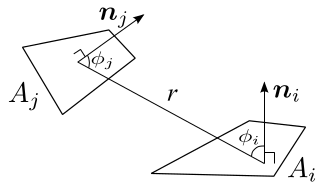
\includegraphics[scale=0.4]{form_factor.png}
    \centering
    \caption{A form factor couples each pair of
    patches}\label{fig:form_factor}
\end{figure}
By assuming $|A_i|\ll r$ and the constancy across patch $A_j$,
we can simplify to the approximate solution
\[
    F_{ij}=\frac{\cos{\phi_i}\cos{\phi_j}|A_j|}{\pi r^2},
\]
giving the \underline{form factor repciprocity}
\[
    F_{ji}=\frac{F_{ij}|A_i|}{|A_j|}
\]
so form factors for only half the patches need to be computed. 
\smallskip
\\But the amount of storage is still massive.
If there are 6e5 patches, there are 3.6e9 form factors and need 7GB.
As many of them are 0 we can save space by using an indexing scheme,
e.g. use 1 bit per form factor, bit=0 indicates form factor=0 and not stored.

\subsection{The Hemicube Method}

\begin{itemize}
    \item \underline{\textbf{Hemicube}}: the half unit cube that bounds the
        hemisphere
        \begin{itemize}
            \item All patches that project onto the same area of the hemisphere have the
                same form factor.
            \item The hemicube is preferred to the hemisphere since computing
                intersections with planes is computationally less demanding.
            \item A hemicube of side 1 unit is placed over the centre of a patch whose
                form factors are to be computed.
            \item Projection of other \emph{nearest visible} patches onto the hemicube 
                could be done by ray tracing (neatly solves occlusion problem)
                or projection (requires z-buffering).
        \end{itemize} 
    \item \underline{\textbf{Hemicube pixels}}: the set of square patches which
        each of the 5 faces of the hemicube is divided regularly into
        \begin{itemize}
            \item the \emph{larger} the size of the hemicube pixel
            \item the \emph{worse} the estimate of the form factors
            \item the \emph{faster} the algorithm
        \end{itemize} 
    \item \underline{\textbf{Delta form factor}}: the form factor between the
        hemicube pixels and the patch under consideration
        \begin{itemize}
            \item If the area of a hemicube pixel is $|A|$, the delta form
                factor is
                \[
                    \frac{\cos{\phi_i}\cos{\phi_j}|A|}{\pi r^2}.
                \]
            \item These delta form factors can be stored in a look-up table.
            \item They can then be applied to each patch without any more form
                factor calculations.
            \item To compute the delta form factors,
                \[
                    \begin{cases}
                        \dfrac{|A|}{\pi r^4} & \text{since for a top face, }
                        \cos{\phi_i}=\cos{\phi_j}=\dfrac{1}{r} \\[8px]
                        \dfrac{z_p|A|}{\pi r^4} & \text{since for a side face, }
                        \cos{\phi_i}=\dfrac{1}{r}, \cos{\phi_j}=\dfrac{z_p}{r}
                    \end{cases}  
                \]
                where $z_p$ is the height of the side face relative to the
                patch.
            \item Once we found the projection of patches, we compute the form
                factor for each patch by summing the delta form factors of the
                hemicube pixels to which it projects.
        \end{itemize} 
\end{itemize} 

\subsection{Meshing}

\begin{itemize}
    \item \underline{\textbf{Meshing}}: the process of dividing the scene into
        patches
    \item Meshing artefacts are scene dependent.
    \item The most obvious are called $D^0$ artefacts, caused by discontinuities
        in the radiosity function.
    \item \underline{\textbf{Discontinuity Meshing}} (\emph{a priori})
        \begin{itemize}
            \item compute discontinuities in advance, e.g. object boundaries,
                albedo/reflectivity discontinuities, shadows, etc.
            \item align the patches with them and don't interpolate them so that
                it is not smoothened
        \end{itemize} 
    \item \underline{\textbf{Adaptive Meshing}} (\emph{a posteriori})
        \begin{itemize}
            \item re-compute the mesh during the radiosity calculation
            \item if two adjacent patches have a strong discontinuity in
                radiosity value, we can
                \begin{itemize}
                    \item put more patches into areas with high discontinuity OR
                    \item move the mesh boundary to coincide with the greatest
                        change
                \end{itemize} 
        \end{itemize} 
    \item \underline{\textbf{h-refinement}}: subdivision of patches
        \begin{enumerate}
            \item Compute the radiosity at the vertices of the coarse grid.
            \item Subvdivide patches if the discontinuities exceed a threshold.
            \item not needed to re-compute complete radiosity by assuming that
            radiosity of a patch is the sum of that of its elements
    \end{enumerate} 
    \item \underline{\textbf{r-refinement}}: patch refinement
        \begin{enumerate}
            \item Compute the radiosity at the vertices of the coarse grid.
            \item Move the patch boundaries closer together if they have high
                radiosity changes.
            \item Need to re-compute the entire radiosity solution for each
                refinement.
        \end{enumerate} 
        \begin{figure}
          	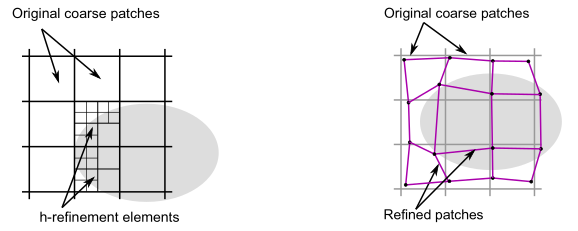
\includegraphics[scale=0.5]{rh-refinement.png}
          	\centering
          	\caption{Adaptive Meshing using h-refinement on the
            left; \\adaptive meshing using r-refinement on the right}
            \label{fig:rh}
        \end{figure}
\end{itemize} 

\subsection{Radiosity Method and Issues}

\begin{enumerate}
    \item Divide the graphics world into discrete patches. \\
        \emph{Meshing strategies, meshing errors}
    \item Compute form factors by the hemicube method. \\
        \emph{Alias errors} 
        \begin{itemize}
            \item due to discrete sampling of a continuous
                environment
            \item not significant since the errors are averaged over a large
                number of pixels
        \end{itemize} 
    \item Solve the matrix equation for the radiosity of each patch. \\
        \emph{Computational strategies} 
        --- see parts regarding Guass Seidle method
    \item Average the radiosity values at the corners of each patch. \\
        \emph{Interpolation approximations}
        \begin{itemize}
            \item may not be significant for small patches
        \end{itemize} 
    \item Compute a texture map of each point or render directly. \\
        \emph{At least this stage is relatively easy!}
\end{enumerate} 


\end{document}
